\section*{Exercice 179 -- Torseur des actions mécaniques transmissibles dans un coussinet}
\setcounter{exo}{0}

\ifprof
\else
Un coussinet (ou bague) est un élément technologique permettant de réaliser des liaisons pivot. Suivant les cas d'utilisation d'un système, un chargement sur l'arbre est transmis au coussinet. 

\begin{center}
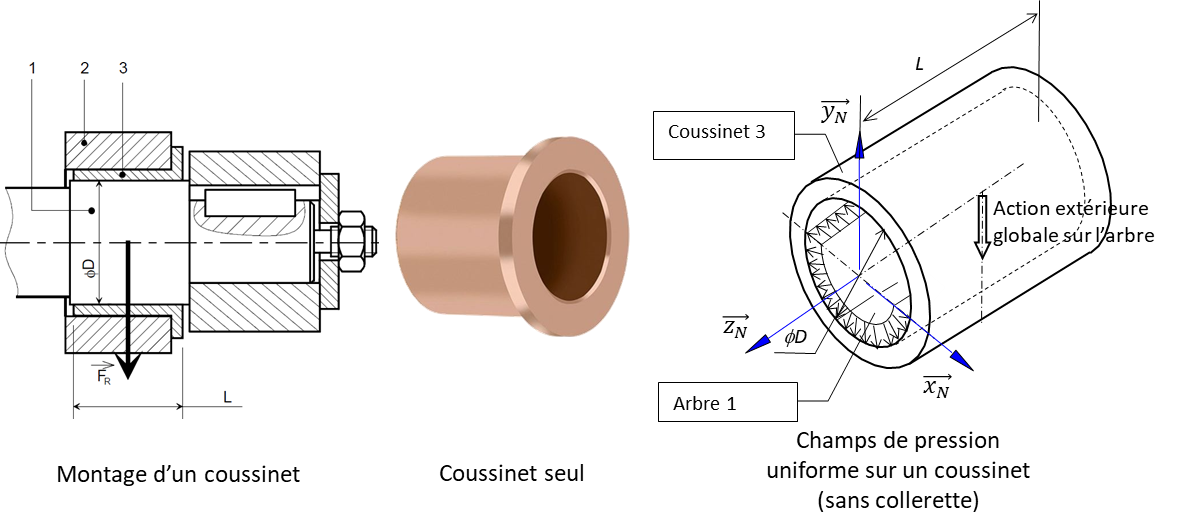
\includegraphics[width=\linewidth]{040_01}
%\textit{}
\end{center}


On donne le modèle suivant où le champ de pression de l'arbre sur le coussinet est uniforme pour $\theta\in[\pi,2\pi]$ 
On note $R=\dfrac{D}{2}$ le rayon du coussinet. 

\begin{center}
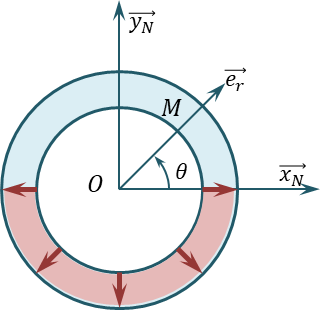
\includegraphics[width=.4\linewidth]{040_02}
%\textit{}
\end{center}
\fi

\subparagraph{}\textit{Déterminer la résultante des actions mécaniques de 1 sur 3. On la note $\vectf{1}{3}$.}
\ifprof
\begin{corrige}
\begin{enumerate}
\item On commence par exprimer le modèle local d'une action mécanique en $M$ : $\dd \vectf{1}{3} = p(M) \dd S \vect{e_r}$.
\item La pression étant uniforme, on a $p(M)=p$.
\item La géométrie du coussinet étant cylindrique, on se place en coordonnées cylindriques et $\dd S = R\dd \theta \dd z$.  
\item $\theta$ varie sur $[\pi, 2\pi]$ et $z$ sur $[0,L]$. 
\item $\vect{e_r}=\cos\theta\vect{x}+\sin\theta\vect{y}$.
\end{enumerate}
Au final, $\vectf{1}{3}=\int p  \left( \cos\theta\vect{x}+\sin\theta\vect{y}\right)R\dd \theta \dd z$
$=pR\int \left( \cos\theta\vect{x}+\sin\theta\vect{y}\right)\dd \theta \dd z$

$=pR\left( \int  \cos\theta\dd \theta \dd z \vect{x}+\int \sin\theta\dd \theta \dd z   \vect{y}\right)$
$=LpR\left( \int  \cos\theta\dd \theta  \vect{x}+\int \sin\theta\dd \theta   \vect{y}\right)$

$=LpR\left( \left[ \sin \theta \right]^{2\pi}_{\pi}  \vect{x}-\left[\cos \theta \right]^{2\pi}_{\pi}   \vect{y}\right)$

$=LpR\left( -(1-(-1))   \vect{y}\right)$

$=LpR\left( -(1-(-1))   \vect{y}\right)$ $=-2LpR   \vect{y}$ $=-LDp   \vect{y}$.

\end{corrige}
\else
\fi


\subparagraph{}\textit{Déterminer $\vectm{O}{1}{3}\vect{z_N}$.}
\ifprof
\begin{corrige}
\begin{enumerate}
\item On commence par exprimer le modèle local d'une action mécanique en $M$ : $\dd \vectf{1}{3} = p(M) \dd S \vect{e_r}$.
\item Au point $O$, on a $\dd \vectm{O}{1}{3}=\vect{OM}\wedge \dd \vectf{1}{3} =\vect{OM}\wedge \dd \vectf{1}{3} $
\item $\vect{OM}=R\vect{e_r}+z\vect{z}$.
\end{enumerate}
On a alors, $ \vectm{0}{1}{3}\vect{z} =\left( \vect{OM}\wedge \dd \vectf{1}{3}\right) \vect{z}$

$ = \left( \left( R\vect{e_r}+z\vect{z} \right) \wedge  p(M) \dd S \vect{e_r}\right) \vect{z}$

$ = \left(z\vect{z} \wedge  p(M) \dd S \vect{e_r}\right) \vect{z} = 0$


\textbf{Rappel :} le produit mixte est invariant par permutation circulaire : $\left( \vect{a}\wedge \vect{b}\right)\cdot \vect{c} = \left( \vect{c}\wedge \vect{a}\right)\cdot \vect{b} = \left( \vect{b}\wedge \vect{c}\right)\cdot \vect{a}$.
\end{corrige}
\else
\fi

\vspace{.5cm}

On considère maintenant que la pression n'est pas uniforme et vaut au point $M$ $p(M)=p_0\sin\theta$.
\subparagraph{}\textit{Justifier que  $\vectf{1}{3}$ n'a une composante que sur $\vect{y}$.}
\ifprof
\begin{corrige}
Pour des raisons de symétrie du champ de pression, la seule composante sera sur $\vect{y_N}$.
\end{corrige}
\else
\fi


\subparagraph{}\textit{Déterminer la résultante des actions mécaniques de 1 sur 3. On la note $\vectf{1}{3}$. On rappelle que $\sin^2\theta =\dfrac{1-\cos 2\theta }{2}$. }
\ifprof
\begin{corrige}
On cherche donc $\vectf{1}{3} \cdot \vect{y_N}$.
\begin{enumerate}
\item On commence par exprimer le modèle local d'une action mécanique en $M$ : $\dd \vectf{1}{3} = p(M) \dd S \vect{e_r}$.
\item La pression étant uniforme, on a $p(M)=p_0 \sin\theta$.
\item La géométrie du coussinet étant cylindrique, on se place en coordonnées cylindriques et $\dd S = R\dd \theta \dd z$.  
\item $\theta$ varie sur $[\pi, 2\pi]$ et $z$ sur $[0,L]$. 
\end{enumerate}

On a  $\dd \vectf{1}{3} \cdot \vect{y_N} = p(M) \dd S \vect{e_r} \cdot \vect{y_N} =p_0 \dd S  \sin^2 \theta $. 

On a donc $\vectf{1}{3} \cdot \vect{y_N} = \int  p_0  \sin^2 \theta  R\dd \theta \dd z $
$ =   p_0 R L \int \dfrac{1-\cos 2\theta }{2}   \dd \theta$
$ =   \dfrac{1}{2}p_0 R L \left[\theta-\dfrac{1}{2}\sin 2\theta \right]^{2\pi}_{\pi} $
$ =   \dfrac{1}{2}p_0 R L {\pi} $
$ =   \dfrac{1}{4}p_0 D L {\pi} $.
\end{corrige}
\else
\fi

\noindent\footnotesize
\fbox{\parbox{.9\linewidth}{
Éléments de corrigé : 
\begin{multicols}{2}
\begin{enumerate}
 \item $\vectf{1}{3}=-LDp   \vect{y}$.
  \item $\vectm{O}{1}{3}\vect{z_N}=0$.
   \item 
    \item $\vectf{1}{3} \cdot \vect{y_N} =-\dfrac{p_0 D L {\pi} }{4}$.
\end{enumerate}
\end{multicols}}}
\normalsize

\ifprof
\newpage
\else
\fi